\question {
    多个线程的规约(Reduce)操作是把每个线程的结果按照某种运算(符合交换律和结合律)两两合并直到得到最终结果的过程。
}

试设计管程{\tt monitor}实现一个$8$线程规约的过程,随机初始化$16$个整数,每个线程通过调用{\tt monitor.getTask}获得$2$个数,相加后,返回一个数{\tt monitor.putResult},然后再{\tt getTask()}直到全部完成退出,最后打印归约过程和结果。

要求: 为了模拟不均衡性,每个加法操作要加上随机的时间扰动,变动区间$1 \sim 10ms$。

提示: 使用{\tt  pthread_}系列的{\tt cond_wait},{\tt cond_signal},{\tt mutex}实现管程;使用{\tt rand()}函数产生随机数,和随机执行时间。

\begin{solution}

代码如下所示:

\lstinputlisting[language=C]{code/monitor.c}

最终输出结果如下:

\begin{figure}[H]
    \centering
    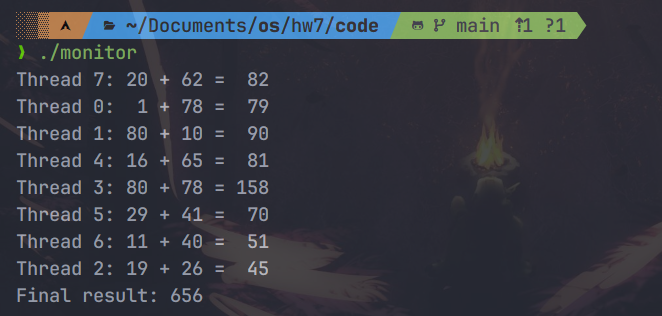
\includegraphics[width=0.8\textwidth]{img/monitor.png}
\end{figure}

\end{solution}
